\chapter{Two-particle momentum probability distribution} \label{app:momDistDer}

\section{Standard form} \label{sec:standardDist}
Derivation of two particle relative momentum probability distribution function.
Starting with the single particle Maxwell-Boltzmann momentum probability distribution function
\begin{equation} 
\label{eq:single_particle_prob}
		 f^1( \vec{p} ) = \left(\frac{1}{2 \pi k_B T}\right)^{3/2} e^{\left(\frac{-p^2}{2 m k_B T}\right)}
\end{equation}
Extension of this simple Boltzmann equation into the two-particle regime can be complicated if their is a dependence of each particle on the others. 
If however, we make the assumption that particle collisions are rapid, we can approximate the two particle momentum distribution as the product of two single particle functions. 
The two particle distribution for a homegeneous system is then
\begin{equation}
\label{eq:two_particle_prob}
\begin{split}
		 f^2( \vec{p}_1, \vec{p}_2 ) &= f^1( \vec{p}_1 ) f^1( \vec{p}_2 ) \\
		  &= \left(\frac{1}{2 \pi m k_B T}\right)^3 \exp{\frac{-(p_1^2 + p_2^2)}{2 m k_B T}}
\end{split}
\end{equation}
Next, we'd like to consider a center-of-mass frame for the distribution. So we'll define
\begin{align*}
	\vec{P}_c & = \vec{p}_1 + \vec{p}_2             &	M   &= m_1 + m_2 = 2m \\
	\vec{p}_r & = \frac{\vec{p}_1 - \vec{p}_2}{2}   &   \mu &= \frac{m_1 m_2}{m_1 + m_2} = \frac{m}{2}
\end{align*}
From these equations we can use conservation of energy to determine the quadrature sum of the two momenta
\begin{align*}
	\frac{p_1^2}{2m} + \frac{p_2^2}{2m} &= \frac{P_c^2}{2M} + \frac{p_r^2}{2\mu} \\
	p_1^2 + p_2^2 &= \frac{P_c^2}{2} + 2 p_r^2
\end{align*}
Thus the momentum probability distribution take the form
\begin{equation} \label{eq:two_particle_prob_inf_atomFrame}
		 f^2( \vec{P}_c, \vec{p}_r ) = \left(\frac{1}{2 \pi M k_B T}\right)^{3/2} \left(\frac{1}{2 \pi \mu k_B T}\right)^{3/2} 
		 \exp{\frac{-P_c^2}{2 M k_B T}} \exp{\frac{-p_r^2}{2 \mu k_B T}}
\end{equation}

\section{Truncated form}\label{sec:truncDist}
Here we'll look at the effects of truncation of the Maxwell-Boltzmann.
Such a system is not in thermal equilibrium and is limited to its truncation value.

Two particle momentum distribution \hl{for correcting notation, use C and R when denoting CoM and Rel}
\begin{equation}
\begin{split}
	f^2_{\vec{r},trunc} (\vec{p}_1, \vec{p}_2) &= A^2 \left(\frac{1}{2 \pi m k_B T}\right)^3 \exp{ \frac{-(p_1^2 + p_2^2)}{2 m k_B T}} \\ &\quad \times \heaviside{\epsilon_{max} - U(\vec{r}) - \frac{p_1^2}{2m}} \heaviside{\epsilon_{max} - U(\vec{r}) - \frac{p_2^2}{2m}}
\end{split}
\end{equation}
We have introduced a normalization constant $A$ here to ensure the that integration over the truncated probability distribution remains equal to one.
The meaning of $_r$ is such that f should be evaluated at each point in space. Furthermore since the atoms are held in a trapping potential, each point in space has a local trap depth relative to the lip at the top of the trap as shown in Fig.\,\ref{fig:haloTrapModel}

We want the distribution of relative momenta so integrate out the center of mass. \hl{Going to drop the two and trunc for now}
\begin{equation}
\begin{split}
	 \tilde{f}_{\vec{r}}(\vec{p}_{rel}) & = \int d^3 \vec{P}_c \; f_{\vec{r}} (\vec{p}_1, \vec{p}_2) \\
	 &= \left(\frac{1}{2 \pi M k_B T}\right)^{3/2} \left(\frac{1}{2 \pi \mu k_B T}\right)^{3/2} A^2 \int d^3 \vec{P}_c \; e^{\left(\frac{-P_c^2}{2 M k_B T}\right)} e^{\left(\frac{-p_r^2}{2 \mu k_B T}\right)} \\ 
	 &\quad \times \; \heaviside{\epsilon_{max} - U(\vec{r}) - \frac{P_c^2}{8m} - \frac{p^2}{2m} - \frac{\vec{P}_c \cdot \vec{p}}{2m}} \heaviside{\epsilon_{max} - U(\vec{r}) - \frac{P_c^2}{8m} - \frac{p^2}{2m} + \frac{\vec{P}_c \cdot \vec{p}}{2m}} 
\end{split}
\end{equation}
Spherically symmetric collisions so can integrate by transforming into spherical coordinates with the radius aligned along the interatomic axis
\begin{equation}
\begin{split}
	 \tilde{f}_{\vec{r}}(\vec{p}) &= \left(\frac{1}{2 \pi M k_B T}\right)^{3/2} \left(\frac{1}{2 \pi \mu k_B T}\right)^{3/2} e^{\left(\frac{-p_r^2}{2 \mu k_B T}\right)} A^2  \int_0^{\pi} \sin \theta d\theta \int_0^{2\pi} d\phi \int_0^{\infty} dP_c \; P_c^2 \; e^{\left(\frac{-P_c^2}{2 M k_B T}\right)} \\ 
	 &\quad \times \; \heaviside{\epsilon_{max} - U(\vec{r}) - \frac{P_c^2}{8m} - \frac{p^2}{2m} - \frac{P_c \, p \cos \theta}{2m}} \heaviside{\epsilon_{max} - U(\vec{r}) - \frac{P_c^2}{8m} - \frac{p^2}{2m} + \frac{P_c \, p \cos \theta}{2m}} 
\end{split}
\end{equation}
Making a change of variables
\begin{equation*}
\begin{split}
	X  &= \cos \theta \\
	dX &= - \sin \theta d \theta
\end{split}
\end{equation*}
Substitute and integrate over $\phi$
\begin{equation}
\begin{split}
	 \tilde{f}_{\vec{r}}(\vec{p}) &= \left(\frac{1}{2 \pi M k_B T}\right)^{3/2} \left(\frac{1}{2 \pi \mu k_B T}\right)^{3/2} e^{\left(\frac{-p_r^2}{2 \mu k_B T}\right)} 2 \pi A^2  \int_{-1}^1 dX \int_0^{\infty} dP_c \; P_c^2 \; e^{\left(\frac{-P_c^2}{2 M k_B T}\right)} \\ 
	 &\quad \times \; \heaviside{\epsilon_{max} - U(\vec{r}) - \frac{P_c^2}{8m} - \frac{p^2}{2m} - \frac{P_c \, p X}{2m}} \heaviside{\epsilon_{max} - U(\vec{r}) - \frac{P_c^2}{8m} - \frac{p^2}{2m} + \frac{P_c \, p X}{2m}} 
\end{split}
\end{equation}
Recognize that the Heaviside functions cancel each other out on either side of zero, so can eliminate one of them and multiply by 2
\begin{equation}
\begin{split}
	 \tilde{f}_{\vec{r}}(\vec{p}) &= \left(\frac{1}{2 \pi M k_B T}\right)^{3/2} \left(\frac{1}{2 \pi \mu k_B T}\right)^{3/2} e^{\left(\frac{-p_r^2}{2 \mu k_B T}\right)} 4 \pi A^2 \int_0^1 dX \int_0^{\infty} dP_c \; P_c^2 \; e^{\left(\frac{-P_c^2}{2 M k_B T}\right)} \\ 
	 &\quad \times \; \heaviside{\epsilon_{max} - U(\vec{r}) - \frac{P_c^2}{8m} - \frac{p^2}{2m} - \frac{P_c \, p X}{2m}} 
\end{split}
\end{equation}
Rewrite using the infinite relative momentum probability distribution $f_{\vec{r}, \infty} (\vec{p})$ from Eq.\,\ref{eq:two_particle_prob_inf_atomFrame}
\begin{equation}
\begin{split}
	 \tilde{f}_{\vec{r}}(\vec{p}) &= \left(\frac{1}{2 \pi \mu k_B T}\right)^{3/2} e^{\left(\frac{-p_r^2}{2 \mu k_B T}\right)} \mathcal{G}(T, \epsilon_{max}, p_{rel}) \\
	 &= f_{\vec{r}, \infty} (\vec{p}) \mathcal{G}(T, \epsilon_{max}, p_{rel})
\end{split}
\end{equation}
where $\mathcal{G}(T, \epsilon_{max}, p_{rel})$ is given by
\begin{equation} \label{eq:mom_dist_st_3}
\begin{split}
	\mathcal{G}(T, \epsilon_{max}, p_{rel}) &= A^2 \left(\frac{4 \pi}{2 \pi M k_B T}\right)^{3/2} \int_0^1 dX \int_0^{\infty} dP_c \; P_c^2 \; e^{\left(\frac{-P_c^2}{2 M k_B T}\right)} \\ 
	 &\quad \times \; \heaviside{\epsilon_{max} - U(\vec{r}) - \frac{P_c^2}{8m} - \frac{p^2}{2m} - \frac{P_c \, p X}{2m}} 
\end{split}
\end{equation}
Now define two dimensionless variables $\tilde{\epsilon}$ and $\tilde{E}$ which will be used to change variables once more
\begin{align*}
	\tilde{\epsilon} &= \frac{p_{rel}^2}{2 \mu k_B T} 												&\quad 		\tilde{E}  &= \frac{P_c^2}{2 M k_B T} \\
	p 				 &= \sqrt{2 \mu k_B T \tilde{\epsilon}}    										&\quad  	P_c 	   &= \sqrt{2 M k_B T \tilde{E}} \\
	dp p^2 			 &= \frac{\sqrt{\tilde{\epsilon}}}{2}(2 \mu k_B T)^{3/2} d \tilde{\epsilon} 	&\quad		dP_c \, P_c^2 &= \frac{\sqrt{\tilde{E}}}{2}(2 M k_B T)^{3/2} d \tilde{E}
\end{align*}
Plugging these expressions into Eq.\ref{eq:mom_dist_st_3} and rearranging
\begin{multline}
	\tilde{f}_{\vec{r}}(\vec{p}) = A^2 \frac{e^{-\tilde{\epsilon}}}{(2 \pi \mu k_B T)^{3/2}} \int_0^1 dX \frac{2}{\sqrt{\pi}} \int_0^\infty d \tilde{E} e^{-\tilde{E}}\sqrt{\tilde{E}} \\
	\times \heaviside{\eta(\vec{r}) - \frac{\tilde{E}}{2} - \frac{\tilde{\epsilon}}{2} - X \sqrt{\tilde{E}\tilde{\epsilon}}}
\end{multline}
would like to turn this distribution into a relative energy distrbution. 
Collisions are isotropic so we can use the relation
\begin{equation}
\begin{split}
	\int dp p^2 \int d \Omega_p \tilde{f}_{\vec{r}}(\vec{p}) = \int d \tilde{\epsilon} \hat{f}_{\vec{r}}(\tilde{\epsilon})) = 1 \\
	\Rightarrow 4 \pi p^2 \tilde{f}_{\vec{r}}(\vec{p}) dp = \hat{f}_{\vec{r}}(\tilde{\epsilon}) d \tilde{\epsilon}
\end{split}
\end{equation}
using $dp p^2$ given above we then write 
\begin{equation} \label{eq:mom_dist_st_4}
	\hat{f}_{\vec{r}}(\tilde{\epsilon}) = A^2 \sqrt{\tilde{\epsilon}} \, e^{-\tilde{\epsilon}} \frac{2}{\sqrt{\pi}} \int_0^1 dX \frac{2}{\sqrt{\pi}} \int_0^\infty d \tilde{E} e^{-\tilde{E}}\sqrt{\tilde{E}} \; \heaviside{\eta(\vec{r}) - \frac{\tilde{E}}{2} - \frac{\tilde{\epsilon}}{2} - X \sqrt{\tilde{E}\tilde{\epsilon}}}
\end{equation}
We can now choose the normalization constant $A^2$ using
\begin{equation*}
	\int_0^{2\eta(\vec{r})} d \tilde{\epsilon} \hat{f}_{\vec{r}}(\tilde{\epsilon}) = 1
\end{equation*}
where we have used an energy cutoff of $2 \eta(\vec{r})$ since either particle may have an energy in the range $[0 \rightarrow \eta(\vec{r})]$. 
With the normalization, the complete expression for $\hat{f}_{\vec{r}}(\tilde{\epsilon})$ is then
\begin{equation}
	\hat{f}_{\vec{r}}(\tilde{\epsilon}) = \frac{2}{\sqrt{\pi}} \sqrt{\tilde{\epsilon}} \, e^{-\tilde{\epsilon}} \hat{\mathcal{G}}(\eta_{\vec{r}}, \tilde{\epsilon})
\end{equation}
where all the effects of the truncation have been moved to $\hat{\mathcal{G}}$, given by 
\begin{equation*}
	\hat{\mathcal{G}}(\eta_{\vec{r}}, \tilde{\epsilon}) = \frac{\displaystyle
	\int_0^1 dX \frac{2}{\sqrt{\pi}} \int_0^\infty d \tilde{E} e^{-\tilde{E}}\sqrt{\tilde{E}} \; \heaviside{\eta(\vec{r}) - \frac{\tilde{E}}{2} - \frac{\tilde{\epsilon}}{2} - X \sqrt{\tilde{E}\tilde{\epsilon}}}}
	{\displaystyle \int_0^{2\eta(\vec{r})} d \tilde{\epsilon} \frac{2}{\sqrt{\pi}} \sqrt{\tilde{\epsilon}} \, e^{-\tilde{\epsilon}} \int_0^1 dX \frac{2}{\sqrt{\pi}} \int_0^\infty d \tilde{E} e^{-\tilde{E}}\sqrt{\tilde{E}} \; \heaviside{\eta(\vec{r}) - \frac{\tilde{E}}{2} - \frac{\tilde{\epsilon}}{2} - X \sqrt{\tilde{E}\tilde{\epsilon}}}}
\end{equation*}
we can check the limiting behavior of this equation since we expect when $$\lim_{\eta \rightarrow \infty} \hat{\mathcal{G}}(\eta_{\vec{r}}, \tilde{\epsilon}) = 1$$. 
Using $$ \int_0^{\infty} dx \sqrt{x} e^{-x} = \frac{\sqrt{\pi}}{2}$$ then this requirement is fulfilled. 


\begin{figure}
\label{fig:momSurfRelCol}
	\centerline{
	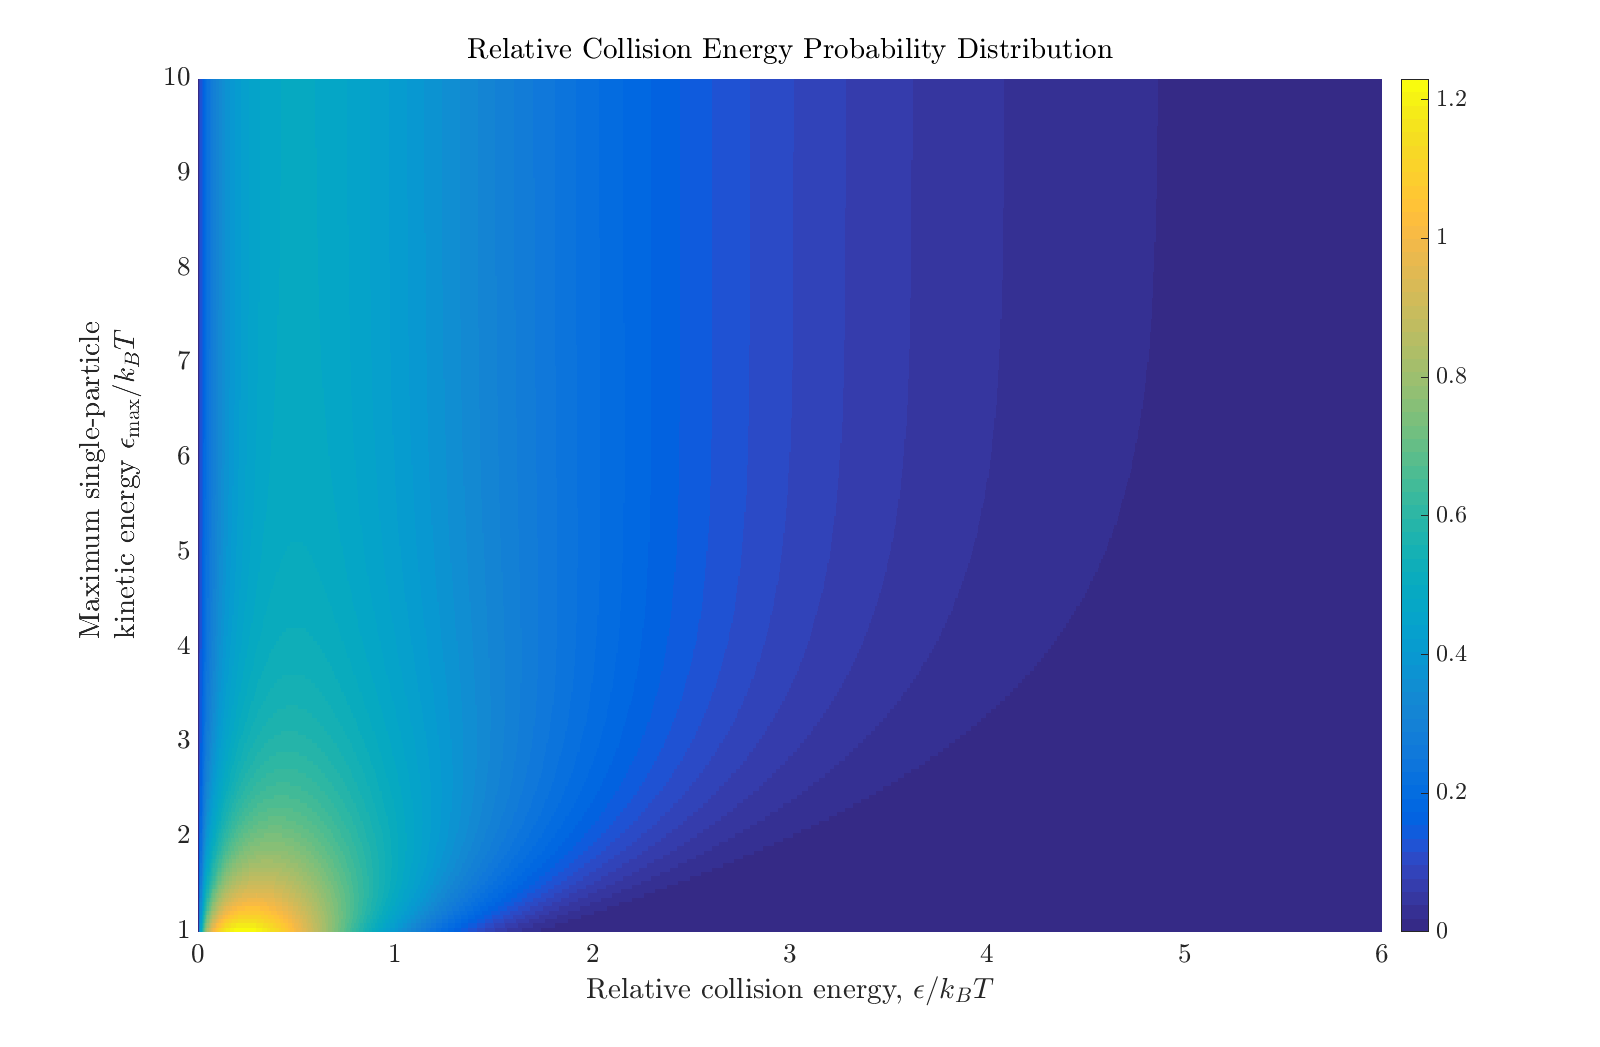
\includegraphics[width=\textwidth]{relativeColDistribution.png}}
	\caption{2D Surface plot of the relative collision likelihood}{}
\end{figure} 
\begin{figure}
\label{fig:momSurfRelCol}
	\centerline{
	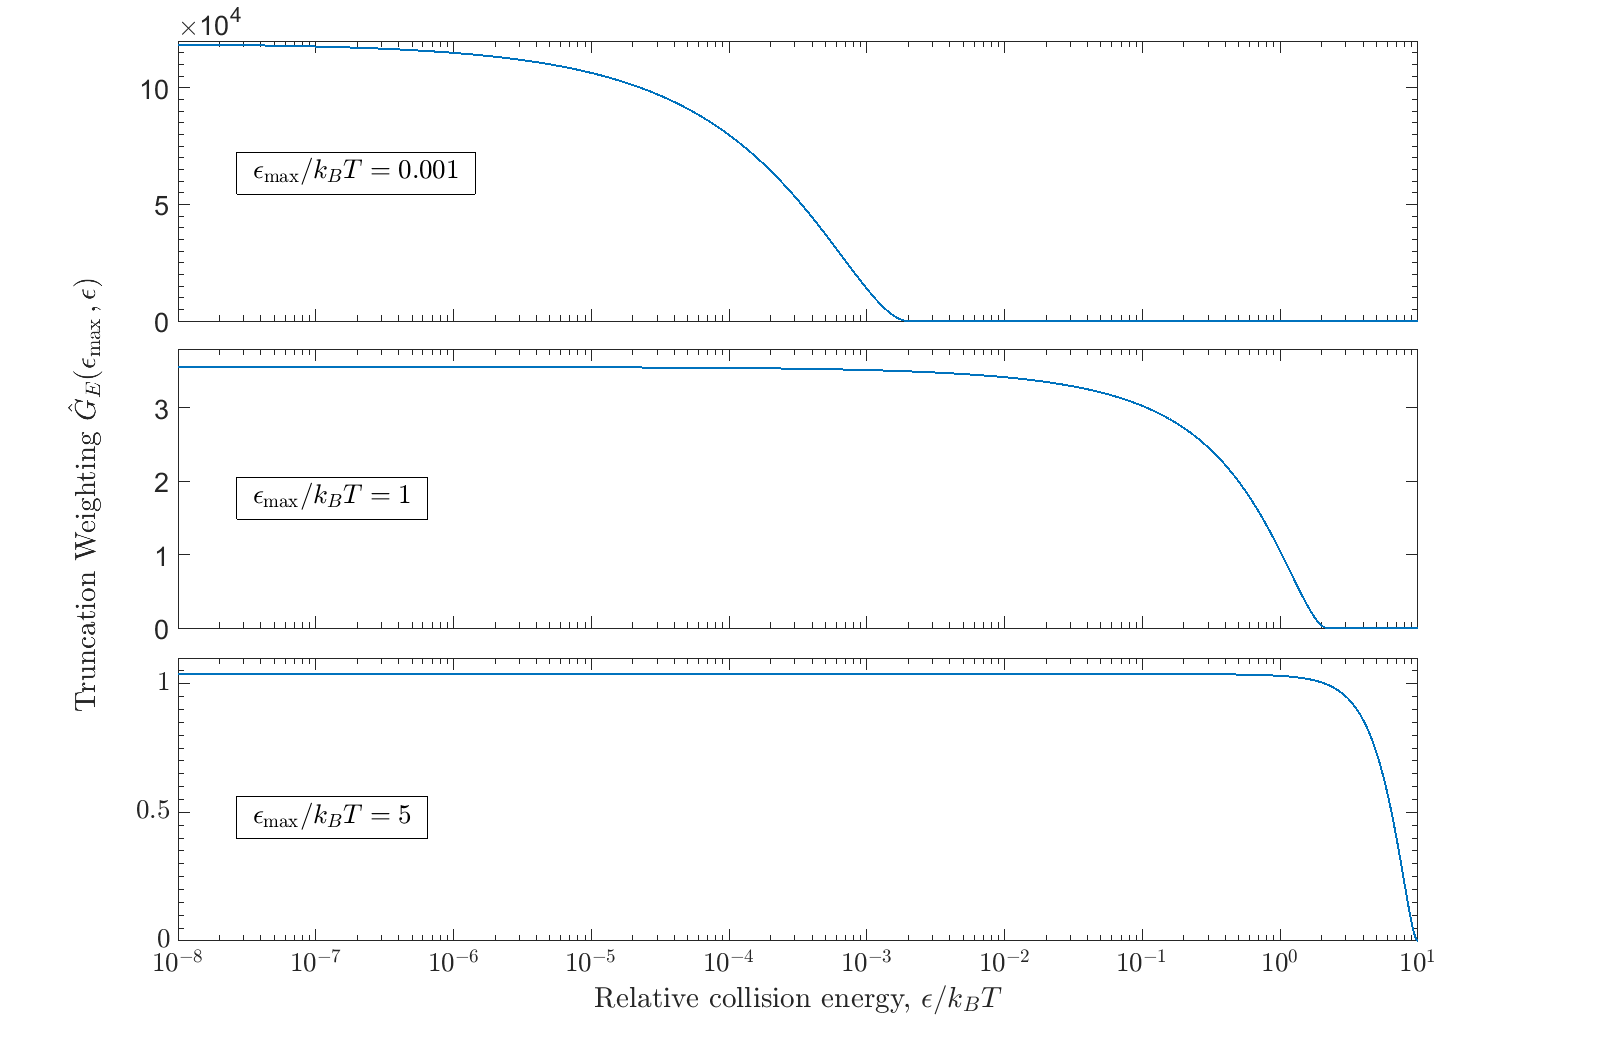
\includegraphics[width=\textwidth]{cutAcrossColE.png}}
	\caption{Behavior of $G(\epsilon,\eta)$ vs. collision energy}{}
\end{figure} 
\begin{figure}
\label{fig:momSurfRelCol}
	\centerline{
	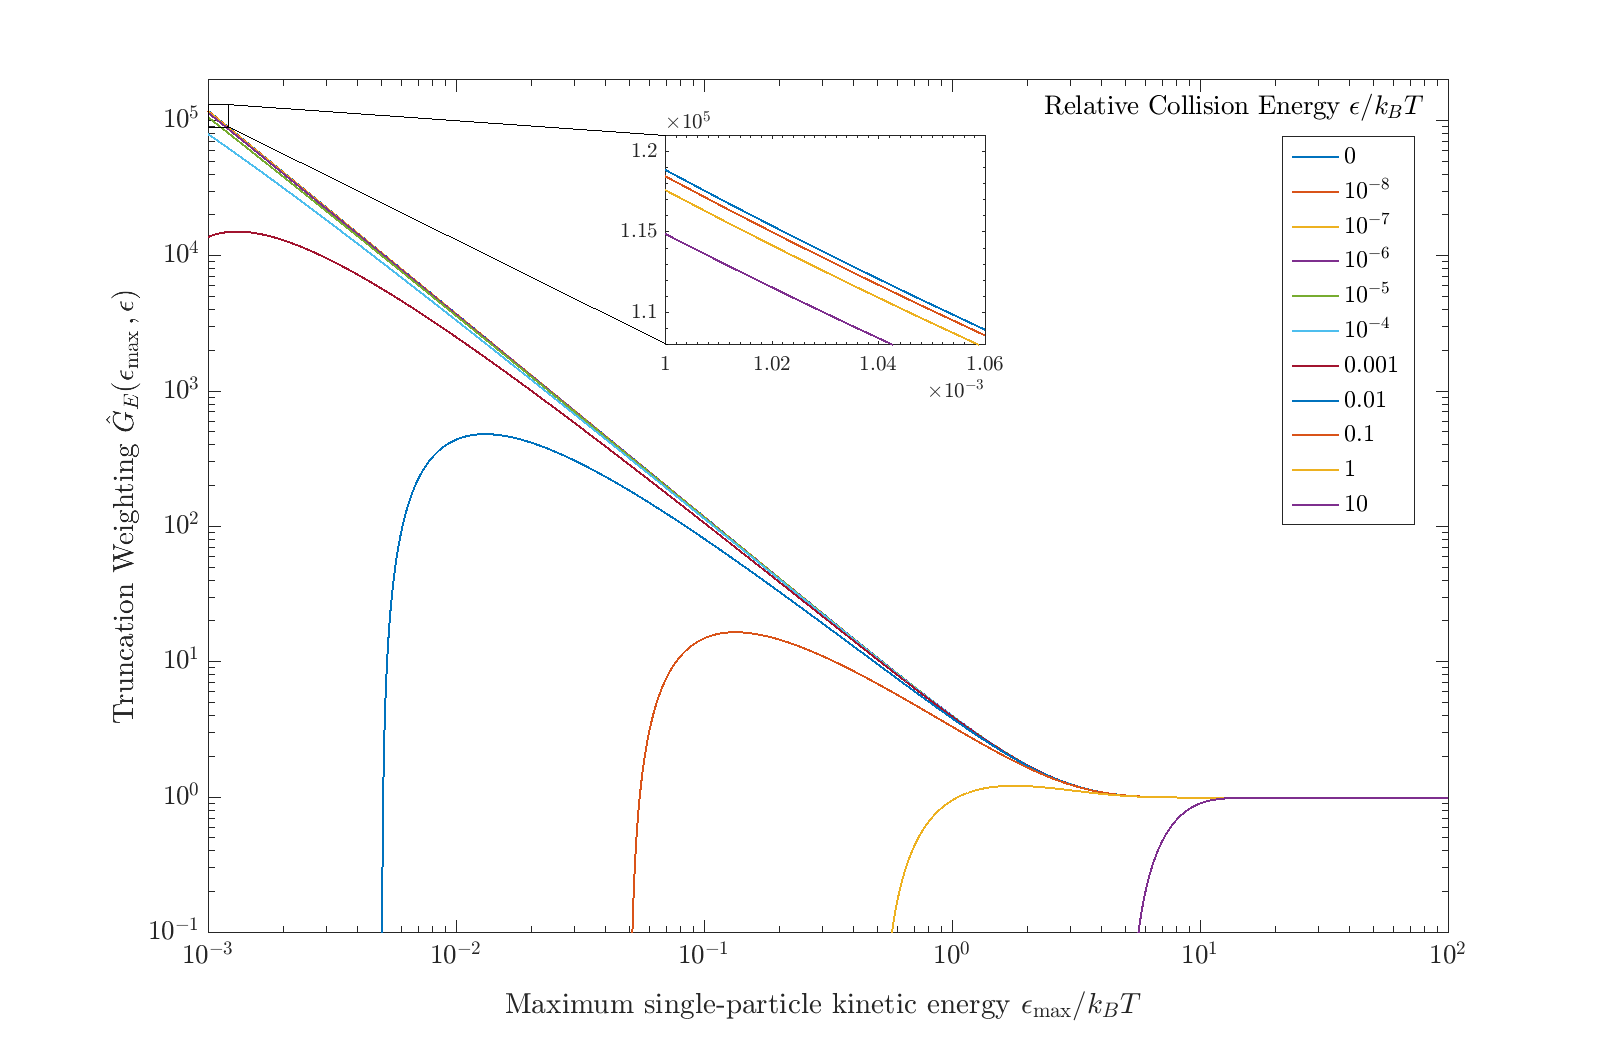
\includegraphics[width=\textwidth]{cutAcrossEta.png}}
	\caption{Behavior of $G(\epsilon,\eta)$ vs. $\eta$}{}
\end{figure} 



